\scanpage{58}
\mspage{28}
\deleted{\unsure{(71)}} et. l'action de $\Gamma_{\underline G}=\Gamma$ sur $\widehat M_G\simeq\widehat M_{g_{\alpha_0},\widehat I_{\alpha_0}}$ est triviale si $g_{\alpha_0}=1$, et elle se fait à travers
\diagram{\begin{tikzcd}[ampersand replacement=\&]
\text{(72)}\quad\Gamma_{\underline G}\arrow[r]\&\unsure{\mathfrak S}_{\widehat I_{\alpha_0}}\quad(\simeq\unsure{\mathfrak S}_4)
\end{tikzcd}}
dans le cas où $g_{\alpha_0}=0$. L'image de $\Gamma_{\underline G}$ dans $\mathfrak S_4$ doit pouvoir être n'importe quel sous-groupe de $\mathfrak S_4$, sauf erreur. Explicitons déjà quels sont les cas où la dim. ambiante est $\leq2$. Le cas de la dim. ambiante $1$ \inserted{i.e. où la codim modulaire \inserted{$s_1$} de $\underline G$ est $0$,} est évidemment celui donné par (70), où $G$ est réduit à un sommet isolé.

Considérons donc le cas de la dim mod ambiante $2$, i.e. codim modulaire $1$, i.e. \uline{une} arête. On trouve soit
\figure{\begin{tikzpicture}[baseline=-.1cm]\draw (0,0) .. controls (.8,.9) and (1.4,-.4) .. (.55,-.3) .. controls (.2,-.2) and (.1,-.1) .. (0,0);\fill (0,0) circle(1.5pt);\node at (1.7,0) {, soit};\draw (2.6,0)--(3.6,0);\draw (2.6,0) circle(1.5pt);\fill (3.6,0) circle(1.5pt);\end{tikzpicture}}.
\inserted{On trouve les trois cas de dim modulaire} \deleted{Dans le cas $g_{\alpha_0}=0$ tous les sommets sauf $1$ sont d'ordre $\unsure{2}$} ambiante $2$, dim. modulaire $1$
\margin{MD-graphes de dim mod $1$, dim. modulaire ambiante $2$.}
\figure{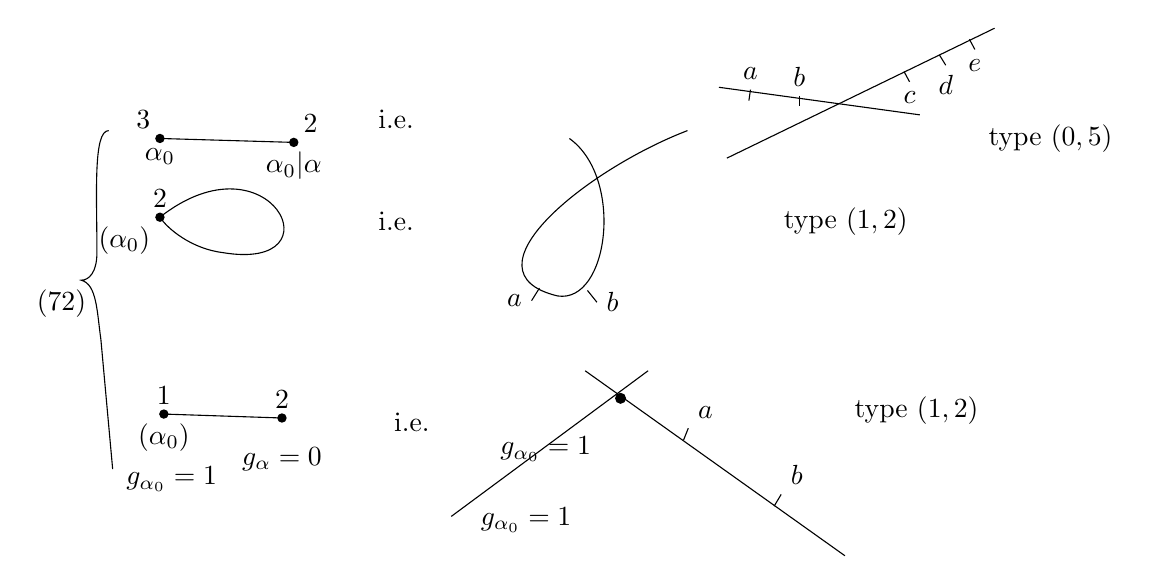
\begin{tikzpicture}[x=1cm,y=1cm]
\node at (-1.25,-1.7) {$(72)$};\draw (-.65,.5) .. controls (-.85,.5) and (-.8,-.3) .. (-.8,-1.05) .. controls (-.8,-1.3) and (-.9,-1.4) .. (-1,-1.4) .. controls (-.8,-1.45) and (-.8,-1.8) .. (-.75,-2.15) -- (-.6,-3.8);
\draw (0,.4)--(1.7,.35);\fill (0,.4) circle(1.7pt);\fill (1.7,.35) circle(1.7pt);\node[above left] at (0,.4) {$3$};\node[below] at (0,.4) {$\alpha_0$};\node[above right] at (1.7,.35) {$2$};\node[below] at (1.7,.35) {$\unsure{\alpha_0|\alpha}$};\node at (3,.65) {i.e.};
\draw (0,-.6) .. controls (1.4,.5) and (2.3,-1.3) .. (.8,-1.05) .. controls (.4,-1) and (.1,-.75) .. (0,-.6);\fill (0,-.6) circle(1.7pt);\node[above] at (0,-.6) {$2$};\node[below left] at (0,-.6) {$(\alpha_0)$};\node at (3,-.65) {i.e.};
\draw (.05,-3.1)--(1.55,-3.15);\fill (.05,-3.1) circle(1.7pt);\fill (1.55,-3.15) circle(1.7pt);\node[above] at (.05,-3.1) {$\deleted{\unsure{1}}$};\node[above] at (1.55,-3.15) {$2$};\node[below] at (.05,-3.1) {$(\alpha_0)$};\node[below] at (.15,-3.65) {$g_{\alpha_0}=1$};\node[below] at (1.55,-3.4) {$g_\alpha=0$};\node at (3.2,-3.2) {i.e.};
\draw (7.1,1.05)--(9.65,.7);\draw (7.2,.15)--(10.6,1.8);\draw (7.5,1.02)--(7.48,.88);\node[above] at (7.5,1.02) {$a$};\draw (8.12,.94)--(8.12,.81);\node[above] at (8.12,.94) {$b$};\draw (9.45,1.25)--(9.52,1.12);\node[below] at (9.52,1.12) {$c$};\draw (9.9,1.46)--(9.98,1.33);\node[below] at (9.98,1.33) {$d$};\draw (10.28,1.66)--(10.35,1.53);\node[below] at (10.35,1.53) {$e$};\node[right] at (10.4,.4) {type $(0,5)$};
\draw (5.2,.4) .. controls (5.9,-.1) and (5.7,-1.7) .. (5.05,-1.6) .. controls (3.8,-1.3) and (5.4,0) .. (6.7,.5);\draw (4.82,-1.5)--(4.72,-1.66);\node[left] at (4.72,-1.66) {$a$};\draw (5.43,-1.53)--(5.55,-1.68);\node[right] at (5.55,-1.68) {$b$};\node[right] at (7.8,-.65) {type $(1,2)$};
\draw (3.7,-4.4)--(6.2,-2.55);\draw (5.4,-2.55)--(8.7,-4.9);\fill (5.85,-2.9) circle(2pt);\node at (4.9,-3.55) {$\deleted{\unsure{g_{\alpha_0}}=1}$};\node at (4.65,-4.45) {$g_{\alpha_0}=1$};\draw (6.65,-3.43)--(6.71,-3.28);\node[above right] at (6.71,-3.28) {$a$};\draw (7.8,-4.27)--(7.89,-4.12);\node[above right] at (7.89,-4.12) {$b$};\node[right] at (8.7,-3.05) {type $(1,2)$};
\end{tikzpicture}}
(NB les sommets, ou branches des courbes, dont le genre \inserted{ou poids marqué} n'est pas marqué en dessous, sont de genre \inserted{ou poids marqué} zéro; les poids marqués sont indiqués sur le graphe \unsure{au|en} dessus des sommets)
\margin{57}
